\begin{frame}
  \frametitle{Hybrid $S_N$-Diffusion Method: Theory}
  \begin{block}{\textbf{New Method for Improved Control Rod Modeling with Neutron Diffusion}}
    \textbf{Hybrid $\bm{S_N}$-Diffusion Method}
    \begin{itemize}
      \item Applies the discrete ordinates ($S_N$) method to a smaller subregion around a
        control rod to generate corrections for the neutron diffusion equation
      \item Limits computationally expensive $S_N$ calculations to small subdomains
      \item Retains the computational efficiency of the neutron diffusion method
    \end{itemize}
  \end{block}
\end{frame}

\begin{frame}
  \frametitle{Hybrid $S_N$-Diffusion Method: Theory}
  \textbf{1-D Discrete Ordinates $\bm{S_N}$ Equation}
  \begin{align}
    \mu_n \frac{d}{dx}&\Psi_g(x, \mu_n) + \Sigma_{t,g}(x)\Psi_g(x, \mu_n) \nonumber \\
                      &=\sum^G_{g'=1} \sum^N_{n'=1} \sum^L_{l=0}
                        \frac{\left(2l+1\right)}{2} \Sigma^{g'\rightarrow g}_{s,l}(x)
                        P_l(\mu_{n'} - \mu_n) w_{n'}\Psi_{g'}(x,\mu_{n'}) \nonumber \\
                      &\qquad + \sum^G_{g'=1} \frac{\chi_g}{2}
                        \frac{\nu\Sigma_{f,g'}(x)}{k} \phi_{g'}(x) + S_g(x,\mu_n)
    \label{eq:1d-sn}
  \end{align}
  \textbf{1-D Neutron Diffusion Equation}
  \begin{align}
    -\frac{d}{dx} D_g(x) \frac{d}{dx} \phi_g(x) + \Sigma_{t,g}(x) \phi_g(x) = \sum^G_{g'=1}&\left[
      \Sigma_s^{g'\rightarrow g}(x)\phi_{g'}(x) + \chi_g\frac{\nu\Sigma_{f,g'}(x)}{k}
    \phi_{g'}(x)\right] \nonumber \\
                                   &+ S_g(x)
    \label{eq:1d-diff}
  \end{align}
\end{frame}

\begin{frame}
  \frametitle{Hybrid $S_N$-Diffusion Method: Theory}
  \textbf{Spatially Varying Diffusion Coefficients (SVDCs)}
  \vspace{.3cm}

  Transport corrections are in the form of \textit{Spatially Varying Diffusion Coefficients
  (SVDCs)}:
  %
  \begin{align}
    D^s_g(x) &= -J^{tr}_g(x)\bigg/\frac{d\phi^{tr}_g(x)}{dx}. \label{eq:svdc}
  \end{align}
  %
  where $D^s$ is the \glspl{SVDC}, and the $tr$ superscript denotes neutron
  current and scalar flux computed from the $S_N$ method. This formulation is similar to the
  space-dependent diffusion coefficients for the Ronen method.
\end{frame}

\begin{frame}
  \frametitle{Hybrid $S_N$-Diffusion Method: Theory}
  \begin{columns}
    \column{.35\textwidth}
    \textbf{Hybrid $S_N$-Diffusion Method Algorithm}
    \vspace{.5cm}

  {\small
  $V_0$: Full problem domain
  \vspace{.1cm}

  $V_1$: Problem subdomain containing control rod region
  \vspace{.1cm}

  $D^s_i$: SVDCs in the $i$-th iteration
\vspace{4cm}}
  \column{.65\textwidth}
  \begin{figure}
    \centering
    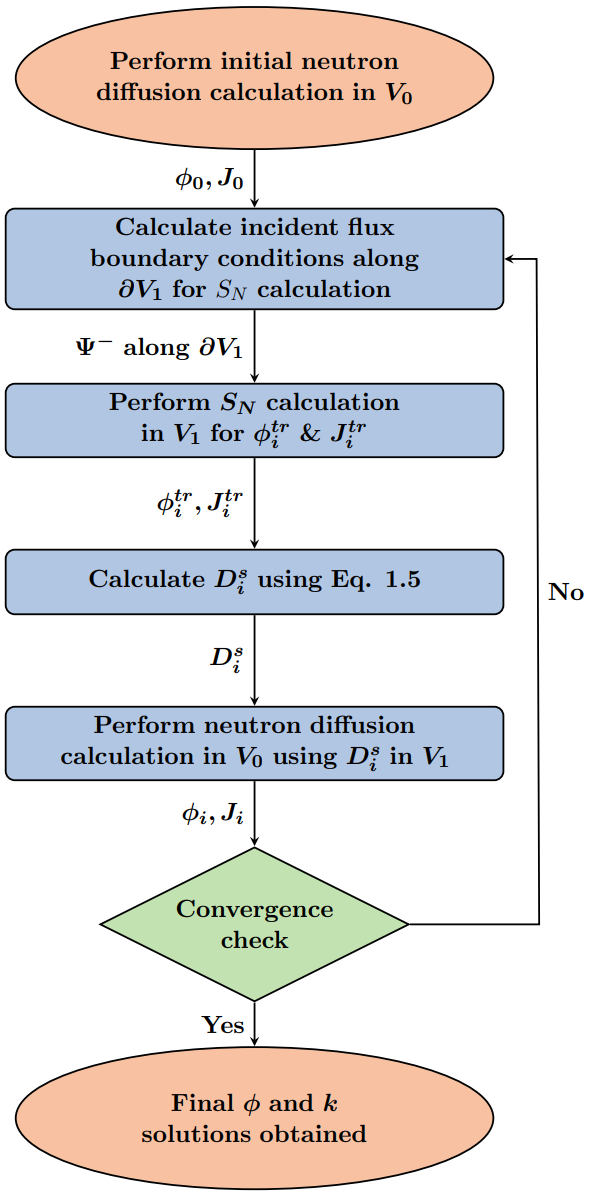
\includegraphics[width=.49\textwidth]{images/algorithm}
    \begin{minipage}[b]{.49\textwidth}
      \caption{Algorithm flowchart for the hybrid $S_N$-diffusion method.}
    \end{minipage}
  \end{figure}
\end{columns}
\end{frame}

\begin{frame}
  \frametitle{Hybrid $S_N$-Diffusion Method: Theory}
  \textbf{$S_N$ Subsolver Boundary Conditions}
  \vspace{.3cm}
  \begin{itemize}
    \item In 1-D, the $S_N$ method requires $N/2$ boundary flux parameters per mesh point.
    \item However, the neutron diffusion method can produce at most one independent parameter per
      mesh point.
    %
    \begin{align}
      J_{g,\pm} &= \frac{\phi_g}{4} \mp \frac{D_g}{2}\frac{d\phi_g}{dx} \label{eq:p1-j}
      \shortintertext{where}
      J_{g,\pm} &= \mbox{ neutron forward/backward current of group }g. \nonumber
    \end{align}
    %
  \end{itemize}
  \pause
  $\Rightarrow$ Assume uniformly isotropic transmission of angular flux:
  %
  \begin{align}
    \Psi_g(x,\mu_n) =& J_{g,+}(x)\Bigg/\sum^N_{n=N/2+1}w_n\mu_n && (\mu_n>0) \\
    \Psi_g(x,\mu_n) =& J_{g,-}(x)\Bigg/\sum^{N/2}_{n=1}w_n\mu_n && (\mu_n<0)
  \end{align}
\end{frame}

\begin{frame}
  \frametitle{Hybrid $S_N$-Diffusion Method: Theory}
  \textbf{Correction Region ($\bm{V_1}$) and Buffer Zone}
  \begin{itemize}
    \item Recall that the full problem domain and the correction region are defined as $V_0$
      and $V_1$, where $V_1 \subseteq V_0$
    \item The approximate $S_N$ boundary conditions will generally yield some deviations in the
      flux distribution since neutron fluxes in realistic reactor systems are at least slightly
      anisotropic in most of the system
    \item However, the influence of boundary conditions on the ratio of $J$ and $\frac{d\phi}{dx}$
      does not extend far from the boundary $\partial V_1$ in optically thick media; SVDCs are
      accurate everywhere except near $\partial V_1$
  \end{itemize}
  \pause
  $\Rightarrow$ Approach for preliminary results: Define $V_1$ such that it is large enough to
  provide sufficient transport
  corrections and accommodate inaccurate SVDCs near $\partial V_1$. Discard inaccurate SVDCs
  in favor of the default $P_1$-based diffusion coefficients.
\end{frame}

